
\section{\textit{Supplementary Material for \cref{subsec:pf}: Results -- Power Flow}}

\subsection{Additional Results on \pfdelta}

\begin{figure}[H]
    \centering
    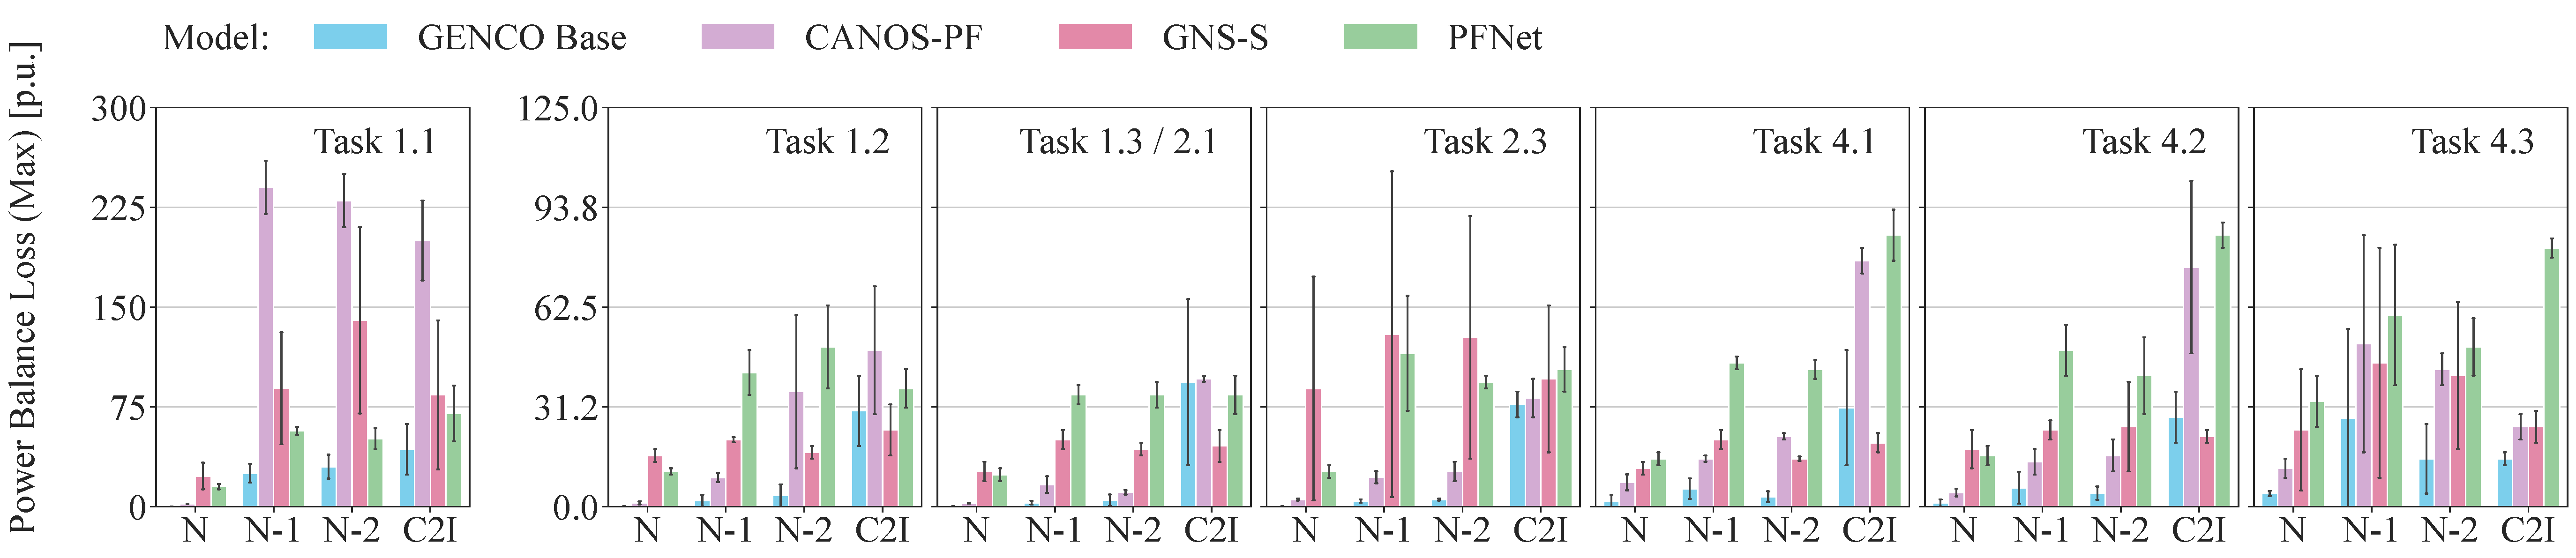
\includegraphics[width=1\columnwidth]{figures/pf_delta/pbl_all_rows_max.pdf}
\caption{Max power-balance loss (computed across all buses of all samples) for \genco, CANOS-PF, GNS-S, and PFNet across PF$\Delta$ tasks on the IEEE 118-bus system. Error bars in the figure correspond to the standard deviation over three seeds. C2I denotes close-to-infeasible cases at the steady-state stability limit, where classical solvers face challenges~\cite{NEURIPS2025_d000ef56}.}
    \label{fig:max-pb}
\end{figure}

\section{\textit{Supplementary Material for \cref{subsec:SE}: Results -- State Estimation}}
\label{app:se}



\begin{figure}[H]
    \centering
    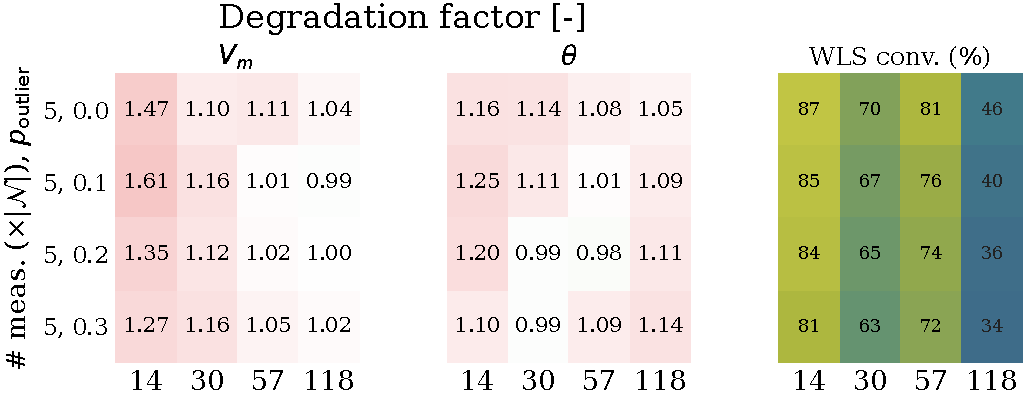
\includegraphics[width=0.7\columnwidth]{figures/se/non_observable.pdf}
    \caption{Degradation in scenarios where WLS did not converge (at a sparse coverage of $5|\mathcal{N}|$ measurements). The first two panels report, for $V_m$ and $\theta$, the ratio of \genco's error on scenarios where the baseline did not converge to its error on scenarios where it did (rows sweep the outlier probability $p_{\text{outlier}}$). Values near $1$ mean \genco is almost as accurate on the hard, non-converged cases as on the easy ones, i.e.\ it degrades gracefully rather than failing outright; values above $1$ indicate higher error on the hard set. The last panel shows the WLS convergence rate. Columns are the IEEE 14-, 30-, 57-, and 118-bus grids.}

    \label{fig:non-observable}
\end{figure}


\section{\textit{Supplementary Material for \cref{subsec:scaling}: Results -- Runtime and Performance Scaling}}
\label{app:runtime_details}


\subsection{Experimental Details}

\paragraph{Grids and sample counts.}
We evaluate small IEEE~14/30/57/118 and large GOC~500/2{,}000/10{,}000 grids. All solvers process the same number of instances per network, respectively:
\[
4\times10^{6},\;
3\times10^{6},\;
2\times10^{6},\;
2\times10^{6},\;
5\times10^{5},\;
5\times10^{4},\;
10^{4}.
\]
Each benchmark run at the selected optimal batch size lasts approximately 20\,s or longer, making initialization operations a small fraction of the measured runtime while keeping the full search for the best batch size or number of workers tractable (runs with suboptimal batch sizes or worker counts can take much longer). All runtime experiments consumed 37.5 H100 GPU-hours for \genco and 343 CPU-node-hours for the PowerModels-based classical solvers.

\paragraph{\genco.}
Inference uses FP32 GPU execution with \texttt{torch.compile(mode="reduce-overhead")}. Each job uses one exclusive H100 80\,GB GPU, 40 CPU cores, and 128\,GB of host RAM; this was sufficient because only $10^4$ samples are resident in memory at once. Batch sizes are powers of two from 64 to 16{,}384 on IEEE grids and from 16 to 16{,}384 on GOC grids. Inference uses 32 DataLoader workers.

\paragraph{Classical solvers implemented through PowerModels.}
AC-PF uses PowerModels' NLsolve-based Newton solver through GOC~500 and a more robust JuMP model on GOC~2{,}000/10{,}000. AC-OPF and DC-OPF use IPOPT with MUMPS; IPOPT uses tolerance $10^{-6}$ and \texttt{max\_iter}=100. Each job is assigned all 84 physical CPU cores of one node, with one Basic Linear Algebra Subprogram (BLAS) thread per worker. The worker sweep is $p\in\{24,40,\ldots,216\}$ (with increments of 16). Reproducing the experiments requires at least 256\,GB for small grids and 960\,GB for large grids. Dispatch batch size is 32 (workers get 32 scenarios to solve at once) on small grids and 1 on large grids to amortize scheduling overhead where solves are cheap without delaying dynamic load balancing on expensive cases.


\subsection{Batch-Size and Worker-Count Sweeps}
\label{appendix:sweep}

\genco's wall-clock time per instance versus batch size for all grids and Base/Small/Tiny models is depicted in \cref{fig:batchsize_vs_runtime_appendix}. Wall-clock time per instance versus worker count for the PowerModels-based classical solvers is shown in \cref{fig:workers_vs_runtime_appendix}. Larger batches or worker pools reduce wall-clock time per instance until saturation; larger models and grids saturate earlier.

\begin{figure}[H]
    \centering
    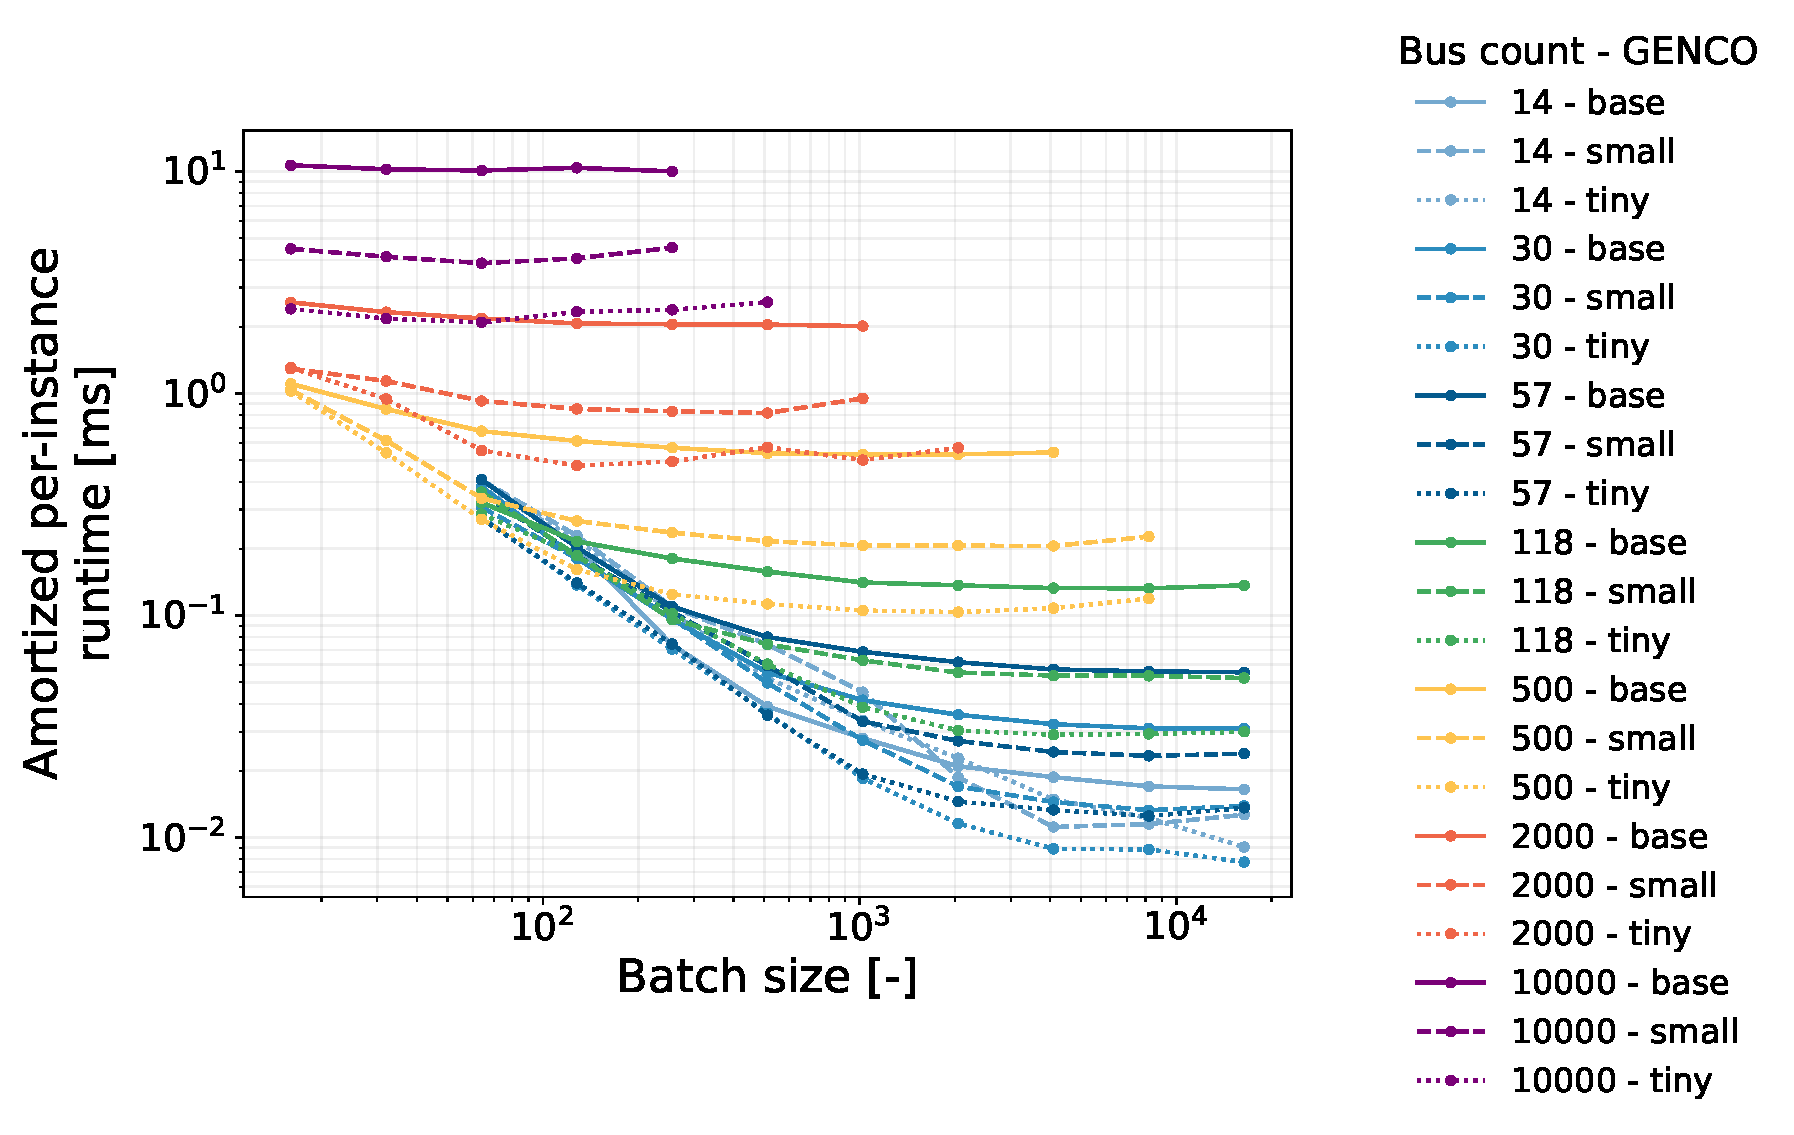
\includegraphics[width=0.5\columnwidth]{figures/runtime_analysis/pf_opf_benchmark_matrix_appendix.pdf}
    \caption{\genco wall-clock time per instance versus batch size across grids and model scales.}
    \label{fig:batchsize_vs_runtime_appendix}
\end{figure}

\begin{figure}[H]
    \centering
    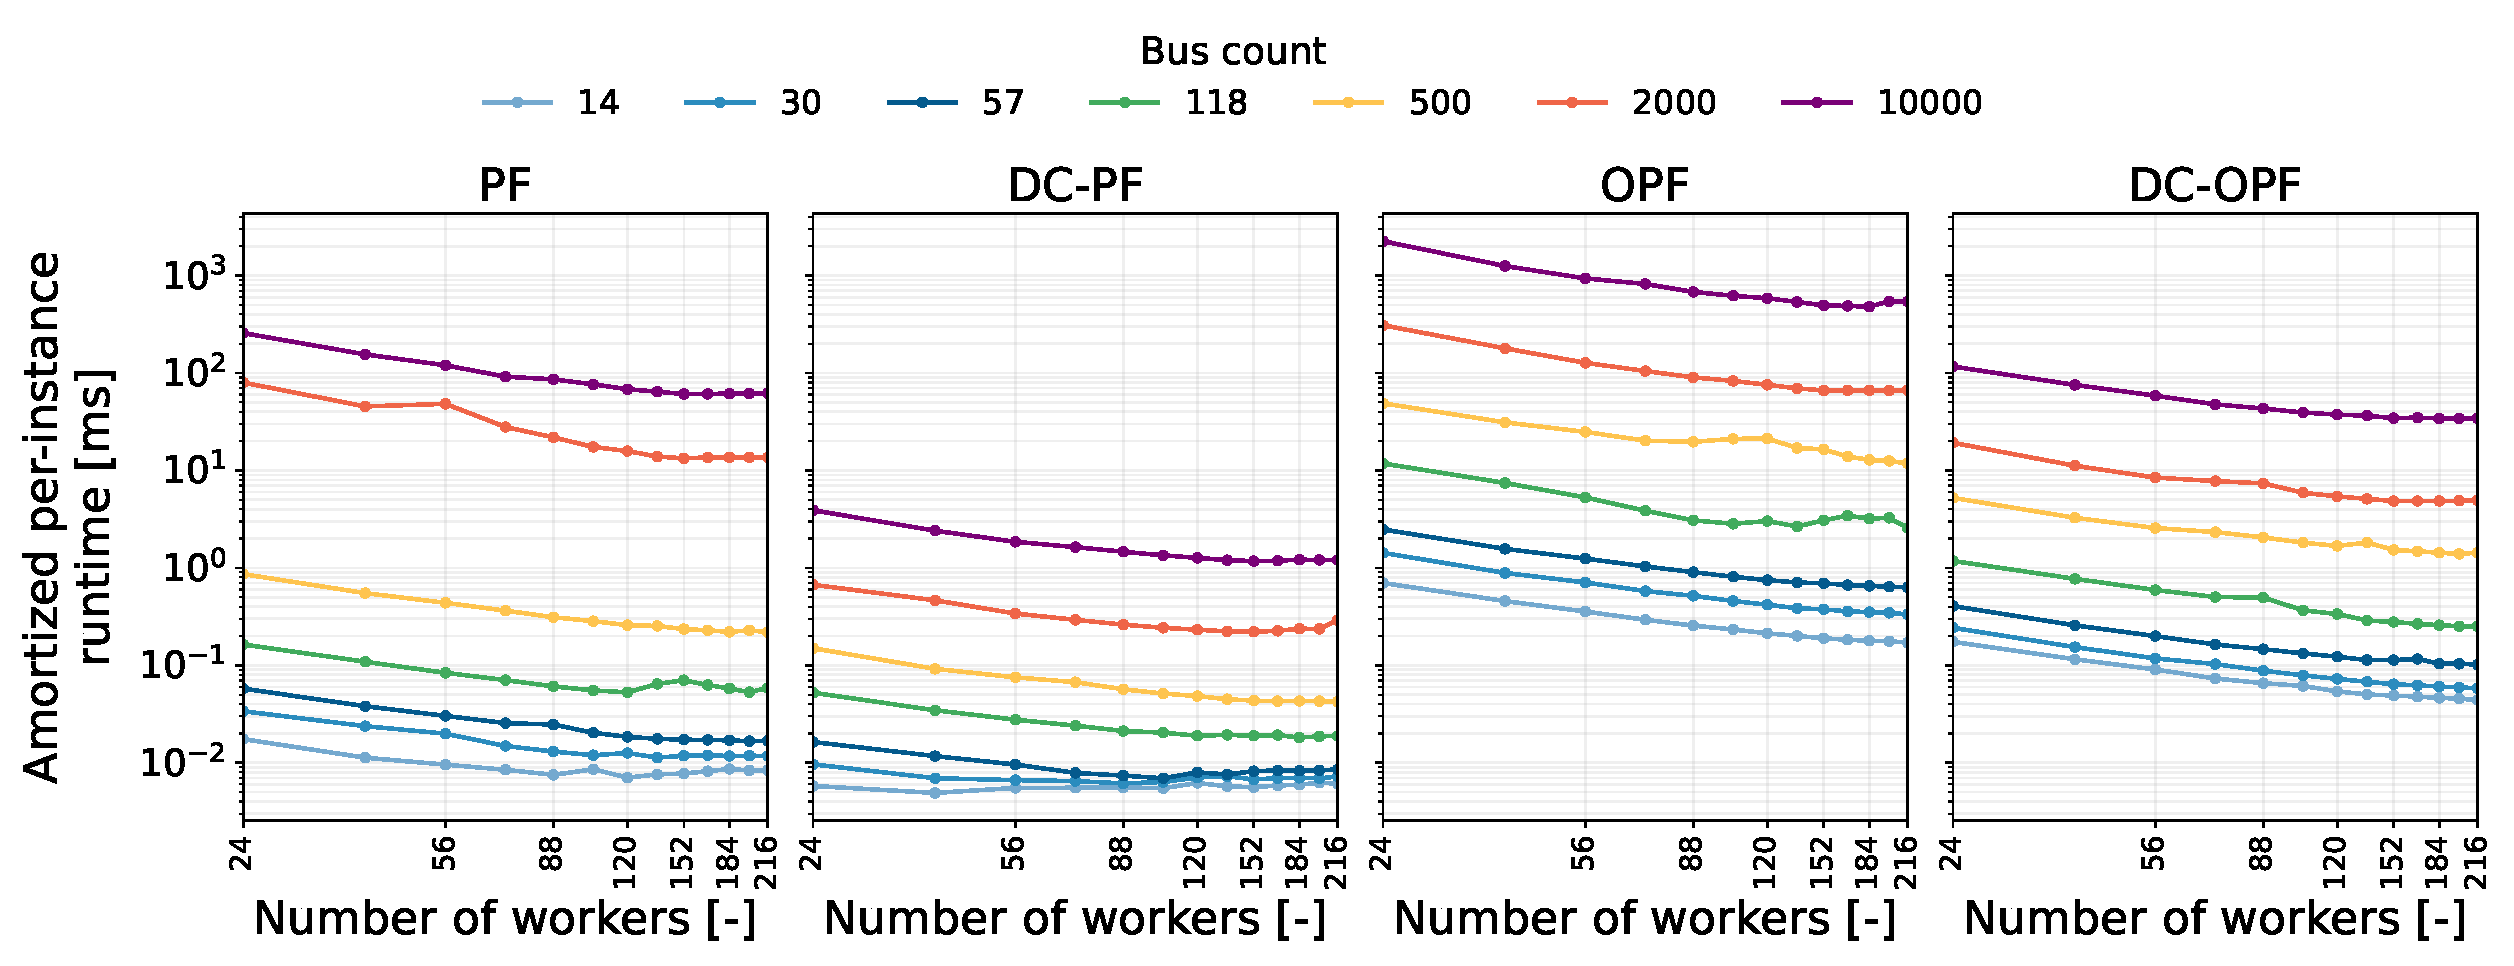
\includegraphics[width=0.7\columnwidth]{figures/runtime_analysis/juliacall_scaling_comparison.pdf}
    \caption{Wall-clock time per instance versus worker count for the PowerModels-based classical AC-PF, DC-PF, AC-OPF, and DC-OPF solvers across grids using the in-memory protocol.}
    \label{fig:workers_vs_runtime_appendix}
\end{figure}


\subsection{Runtime Analysis With and Without Data Loading}
\label{app:s1_vs_s2}

\paragraph{Protocols.}

The main results in \cref{subsec:scaling} use an \emph{in-memory protocol} designed to represent repeated scenario analysis around a reference operating point. The \emph{from-disk protocol} complements this setup by considering grid snapshots in which each scenario is an independent input loaded from disk. The two protocols therefore capture two distinct use cases: repeated in-memory perturbations around a base operating point, and solving heterogeneous scenarios retrieved from storage.

\paragraph{Practical differences.}

In the \emph{in-memory protocol}, both solver classes use preprocessed, parsed, and memory-resident scenarios: GENCO cycles over $10^4$ already loaded tensors in RAM, while each PowerModels worker uses an already parsed base case. The number and content of the tensors do not affect solve runtime; the large pool is used only to avoid potential caching effects. In contrast, in the \emph{from-disk protocol}, both solver classes read scenarios from disk: GENCO reads each processed sample, while PowerModels reads and parses a ready-to-solve \datakit scenario. In both protocols, GENCO uses batched GPU inference and the PowerModels-based classical solvers use multiple CPU workers, with the same parallelization strategy used to maximize throughput. The only difference in timing scope between the two protocols is whether scenario data loading is included in the measured runtime.\\

The from-disk protocol additionally introduces practical dependencies that are absent from the in-memory protocol, including storage format (e.g., JSON versus other representations), scenario access order (e.g., sequential versus non-sequential access), page-cache state, filesystem type (e.g., local node storage versus GPFS), and system contention. Finally, the solved scenarios differ between the two protocols: the in-memory protocol repeatedly solves the fixed base case, whereas the from-disk protocol solves distinct \datakit scenarios. The use of distinct \datakit scenarios is intentional: the from-disk protocol is designed to represent workloads in which heterogeneous grid snapshots are independently retrieved and solved, rather than repeated perturbations around a single operating point. The resulting runtime difference therefore reflects both data-loading overhead and differences in scenario difficulty and should be interpreted as a comparison of two workload regimes.




\paragraph{Observed effects.}

Loading primarily affects \genco's small-grid speedups as shown in \cref{tab:loading_speedups}. Under the from-disk protocol, \genco is slower than AC-PF on IEEE~14/30/57, but remains faster than AC-OPF on every grid; the large-grid conclusions are unchanged.\\

\begin{table}[H]
\centering
\scriptsize
\setlength{\tabcolsep}{5pt}
\caption{\genco Tiny speedups relative to classical AC-PF and AC-OPF solvers. Speedup is classical solvers' wall-clock time per instance divided by \genco wall-clock time per instance; values above one favor \genco.}
\label{tab:loading_speedups}
\begin{tabular}{@{}l cc cc@{}}
\toprule
& \multicolumn{2}{c}{vs.\ AC-PF} & \multicolumn{2}{c}{vs.\ AC-OPF} \\
\cmidrule(lr){2-3}\cmidrule(lr){4-5}
Grid & In-memory & From-disk & In-memory & From-disk \\
\midrule
IEEE 14     & $0.8\times$  & $0.3\times$  & $18.9\times$  & $6.4\times$ \\
IEEE 30     & $1.5\times$  & $0.4\times$  & $43.0\times$  & $9.5\times$ \\
IEEE 57     & $1.3\times$  & $0.6\times$  & $50.4\times$  & $16.1\times$ \\
IEEE 118    & $1.8\times$  & $1.4\times$  & $88.4\times$  & $50.6\times$ \\
GOC 500     & $2.1\times$  & $2.6\times$  & $114.0\times$ & $108.9\times$ \\
GOC 2{,}000 & $28.2\times$ & $31.4\times$ & $140.0\times$ & $160.8\times$ \\
GOC 10{,}000 & $29.1\times$ & $28.9\times$ & $229.1\times$ & $243.0\times$ \\
\bottomrule
\end{tabular}
\end{table}

Loading matters most when computation is inexpensive and becomes negligible as model or grid complexity grows as depicted in \cref{fig:loading_overhead_best_config}. For PowerModels, loading affects DC-PF most on large grids because JSON parsing complexity grows faster with grid size than DC-PF solve complexity; AC-PF changes by only about $1.0$--$1.3\times$, while OPF remains near parity because optimization dominates parsing. Ratios below one coincide with lower mean solve times over diverse scenarios than for the repeated base case, indicating that the base load and topology are harder than the average scenario.


\begin{figure}[H]
    \centering
    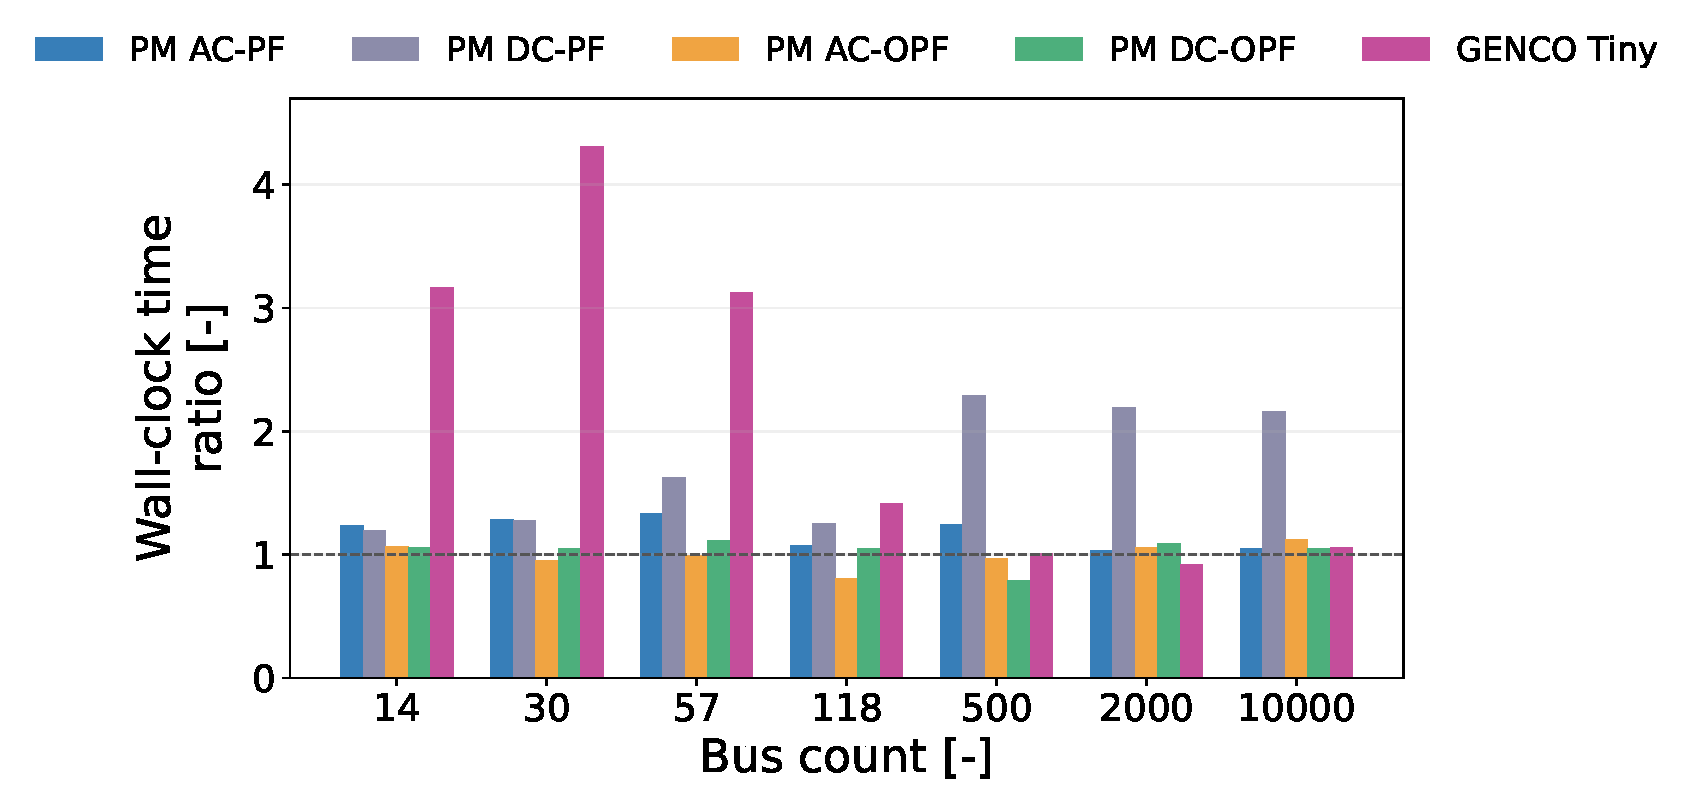
\includegraphics[width=0.5\columnwidth]{figures/runtime_analysis/loading_overhead_best_config.pdf}
    \caption{Ratio of from-disk to in-memory wall-clock time per instance at the best configuration selected independently under each protocol. The dashed line marks equal time; values above one indicate loading overhead.}
    \label{fig:loading_overhead_best_config}
\end{figure}





\subsection{Additional OPF scaling results}

Detailed results for \genco Base and Small from IEEE~14 through GOC~2{,}000 are provided in \cref{tab:opf_scaling}.
\begin{table}[H]
\caption{Constraint violations and optimality gaps for \genco and DC-OPF, with AC-OPF as the optimality reference. Bold entries denote metrics for which the performance difference exceeds one standard deviation. The metrics are computed as described in Section~\ref{subsec:opf}. \genco Base and Small achieve similar feasibility and optimality improvements across all systems.}
\label{tab:opf_scaling}
\centering
\footnotesize
\setlength{\tabcolsep}{4pt}
\begin{tabular}{@{}lllllclll@{}}
\toprule
& & Optimality & \multicolumn{2}{c}{Thermal limits} & \multicolumn{2}{c}{Power balance} & React.\ gen. bounds \\
\cmidrule(lr){3-3}\cmidrule(lr){4-5}\cmidrule(lr){6-7}\cmidrule(lr){8-8}
System & Model
  & Gap (\%)
  & $S_{ij}(+)$ [MVA]
  & $S_{ij}(-)$ [MVA]
  & $\mathrm{PBRes}_{P}$ [MW]
  & $\mathrm{PBRes}_{Q}$ [MVar]
  & $Q_g$ [MVar] \\
\midrule

\multirow{3}{*}{IEEE 14}
  & \genco Base
  & \textbf{0.10 $\pm$ 0.00}
  & 2.56e-5 $\pm$ 1.94e-5
  & 1.32e-5 $\pm$ 2.93e-6
  & \textbf{4.35e-3 $\pm$ 9.46e-5}
  & \textbf{3.79e-3 $\pm$ 1.11e-4}
  & 1.28e-3 $\pm$ 1.57e-4 \\

  & \genco Small
  & 0.10 $\pm$ 0.01
  & 2.46e-5 $\pm$ 1.83e-5
  & 1.37e-5 $\pm$ 2.37e-6
  & 5.51e-3 $\pm$ 5.28e-4
  & 4.63e-3 $\pm$ 6.25e-5
  & \textbf{1.20e-3 $\pm$ 2.44e-4} \\

  & DC-OPF
  & 5.75 $\pm$ 0.01
  & \textbf{0}
  & \textbf{0}
  & 1.42e+0 $\pm$ 4.56e-3
  & --
  & -- \\
\midrule

\multirow{3}{*}{IEEE 30}
  & \genco Base
  & \textbf{0.21 $\pm$ 0.02}
  & 1.13e-3 $\pm$ 1.74e-4
  & \textbf{1.11e-3 $\pm$ 1.55e-4}
  & \textbf{6.90e-3 $\pm$ 1.05e-3}
  & \textbf{4.95e-3 $\pm$ 2.93e-4}
  & \textbf{7.00e-4 $\pm$ 3.11e-4} \\

  & \genco Small
  & 0.25 $\pm$ 0.01
  & \textbf{1.12e-3 $\pm$ 1.94e-4}
  & 1.12e-3 $\pm$ 1.61e-4
  & 1.06e-2 $\pm$ 1.81e-3
  & 8.03e-3 $\pm$ 6.59e-4
  & 8.95e-4 $\pm$ 3.92e-5 \\

  & DC-OPF
  & 7.83 $\pm$ 0.03
  & 9.83e-2 $\pm$ 1.02e-3
  & 7.89e-2 $\pm$ 8.04e-4
  & 6.34e-1 $\pm$ 4.27e-3
  & --
  & -- \\
\midrule

\multirow{3}{*}{IEEE 57}
  & \genco Base
  & 1.21 $\pm$ 0.18
  & 2.89e-3 $\pm$ 3.64e-4
  & 3.04e-3 $\pm$ 6.22e-5
  & 4.13e-1 $\pm$ 1.59e-1
  & 1.80e-1 $\pm$ 7.74e-2
  & \textbf{6.15e-3 $\pm$ 7.11e-4} \\

  & \genco Small
  & \textbf{0.88 $\pm$ 0.14}
  & \textbf{2.69e-3 $\pm$ 5.02e-5}
  & \textbf{2.87e-3 $\pm$ 3.28e-4}
  & \textbf{3.00e-1 $\pm$ 6.92e-2}
  & \textbf{1.62e-1 $\pm$ 3.38e-2}
  & 7.25e-3 $\pm$ 1.28e-3 \\

  & DC-OPF
  & 5.54 $\pm$ 0.02
  & 1.53e-2 $\pm$ 3.36e-4
  & 1.15e-2 $\pm$ 2.26e-4
  & 1.29e+0 $\pm$ 2.51e-3
  & --
  & -- \\
\midrule

\multirow{3}{*}{IEEE 118}
  & \genco Base
  & 1.66 $\pm$ 0.03
  & \textbf{3.75e-2 $\pm$ 5.62e-3}
  & \textbf{3.74e-2 $\pm$ 5.78e-3}
  & 1.36e+0 $\pm$ 1.12e-1
  & 2.75e-1 $\pm$ 2.36e-3
  & 1.19e-3 $\pm$ 6.65e-4 \\

  & \genco Small
  & \textbf{1.66 $\pm$ 0.03}
  & 4.21e-2 $\pm$ 4.48e-5
  & 4.17e-2 $\pm$ 3.73e-4
  & \textbf{1.12e+0 $\pm$ 6.14e-2}
  & \textbf{2.57e-1 $\pm$ 1.49e-2}
  & \textbf{1.13e-3 $\pm$ 1.83e-4} \\

  & DC-OPF
  & 4.73 $\pm$ 0.02
  & 1.04e-1 $\pm$ 6.49e-4
  & 1.06e-1 $\pm$ 6.25e-4
  & 2.46e+0 $\pm$ 3.11e-3
  & --
  & -- \\
\midrule

\multirow{3}{*}{GOC 500}
  & \genco Base
  & \textbf{0.49 $\pm$ 0.08}
  & \textbf{3.83e-3 $\pm$ 3.57e-4}
  & \textbf{3.86e-3 $\pm$ 1.76e-4}
  & \textbf{7.07e-1 $\pm$ 8.16e-2}
  & \textbf{1.89e-1 $\pm$ 2.18e-2}
  & \textbf{4.90e-4 $\pm$ 1.27e-4} \\

  & \genco Small
  & 0.57 $\pm$ 0.01
  & 4.22e-3 $\pm$ 6.91e-6
  & 4.39e-3 $\pm$ 1.76e-4
  & 8.16e-1 $\pm$ 9.95e-3
  & 2.48e-1 $\pm$ 8.65e-3
  & 6.19e-4 $\pm$ 3.00e-5 \\

  & DC-OPF
  & 1.81 $\pm$ 0.01
  & 4.35e-2 $\pm$ 1.47e-4
  & 8.01e-2 $\pm$ 3.20e-5
  & 1.85e+0 $\pm$ 4.12e-3
  & --
  & -- \\
\midrule

\multirow{3}{*}{GOC 2000}
  & \genco Base
  & \textbf{1.53 $\pm$ 0.03}
  & 3.56e-2 $\pm$ 2.35e-2
  & 3.66e-2 $\pm$ 2.49e-2
  & 2.94e+0 $\pm$ 3.05e-1
  & \textbf{7.93e-1 $\pm$ 1.25e-1}
  & \textbf{5.53e-3 $\pm$ 1.56e-3} \\

  & \genco Small
  & 1.54 $\pm$ 0.00
  & \textbf{7.30e-3 $\pm$ 1.04e-3}
  & \textbf{7.56e-3 $\pm$ 7.94e-4}
  & 2.85e+0 $\pm$ 2.37e-1
  & 8.02e-1 $\pm$ 7.62e-2
  & 5.99e-3 $\pm$ 2.16e-3 \\

  & DC-OPF
  & 2.84 $\pm$ 0.02
  & 5.14e-2 $\pm$ 2.76e-4
  & 9.57e-2 $\pm$ 4.37e-4
  & \textbf{1.08e+0 $\pm$ 7.34e-3}
  & --
  & -- \\
\midrule

\bottomrule
\end{tabular}

\raggedright\footnotesize
$\pm$ denotes standard deviation over three seeds.
\end{table}











\section{\textit{Supplementary Material for \cref{subsec:generalization}: Results -- Robustness \& Generalization}}

\label{appendix:top}

The percentage of samples below
absolute active power-balance residual thresholds is shown in \cref{fig:abs_threshold_k10}. It is similar to \cref{fig:threshold_share_relative_k10} but uses absolute thresholds instead of relative ones, and includes buses with zero net injection.\\

The percentage of samples below 1\% residuals as a function of the contingency order is depicted in \cref{fig:rel_threshold_vs_k}.

\begin{figure}[H]
\centering

\begin{minipage}{0.4\linewidth}
\centering
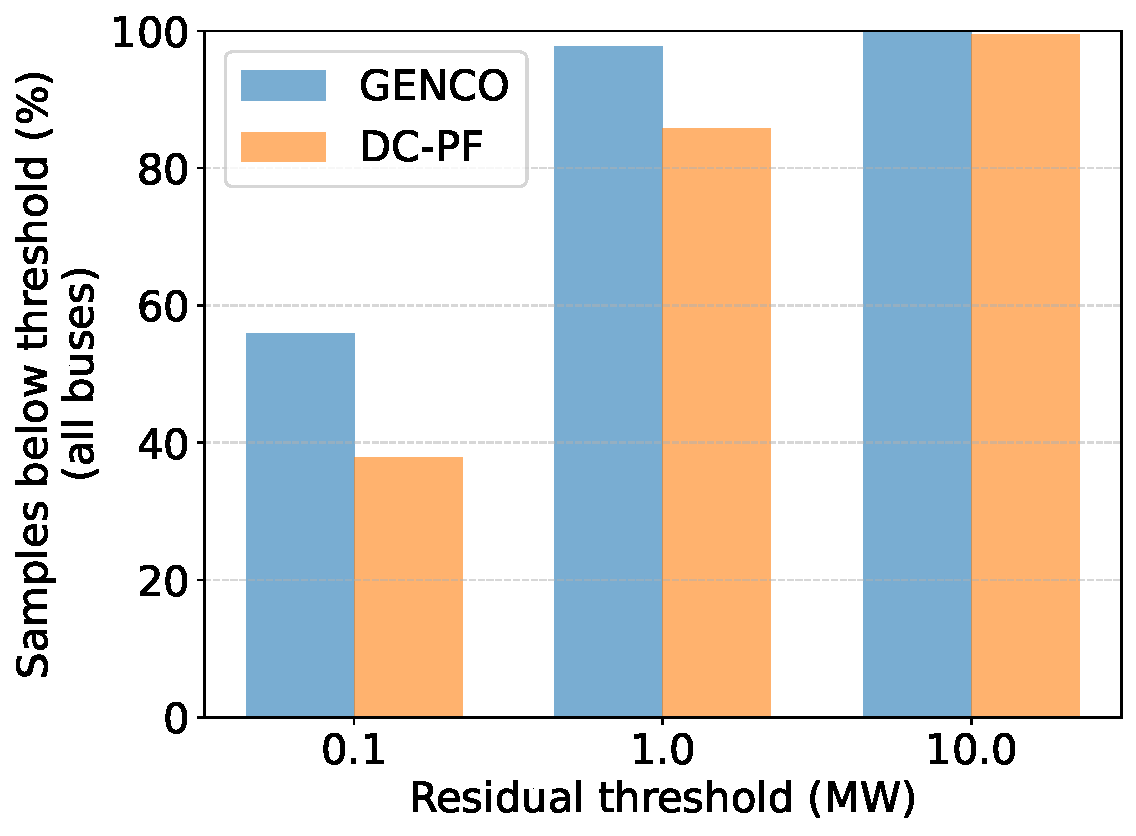
\includegraphics[width=\linewidth]{figures/robustness/threshold_share_absolute_k10.pdf}
\caption{Percentage of samples below absolute active power-balance residual thresholds at $k=10$ (all buses). \genco again dominates DC-PF across all thresholds.}
\label{fig:abs_threshold_k10}
\end{minipage}
\hspace{3cm}
\begin{minipage}{0.4\linewidth}
\centering
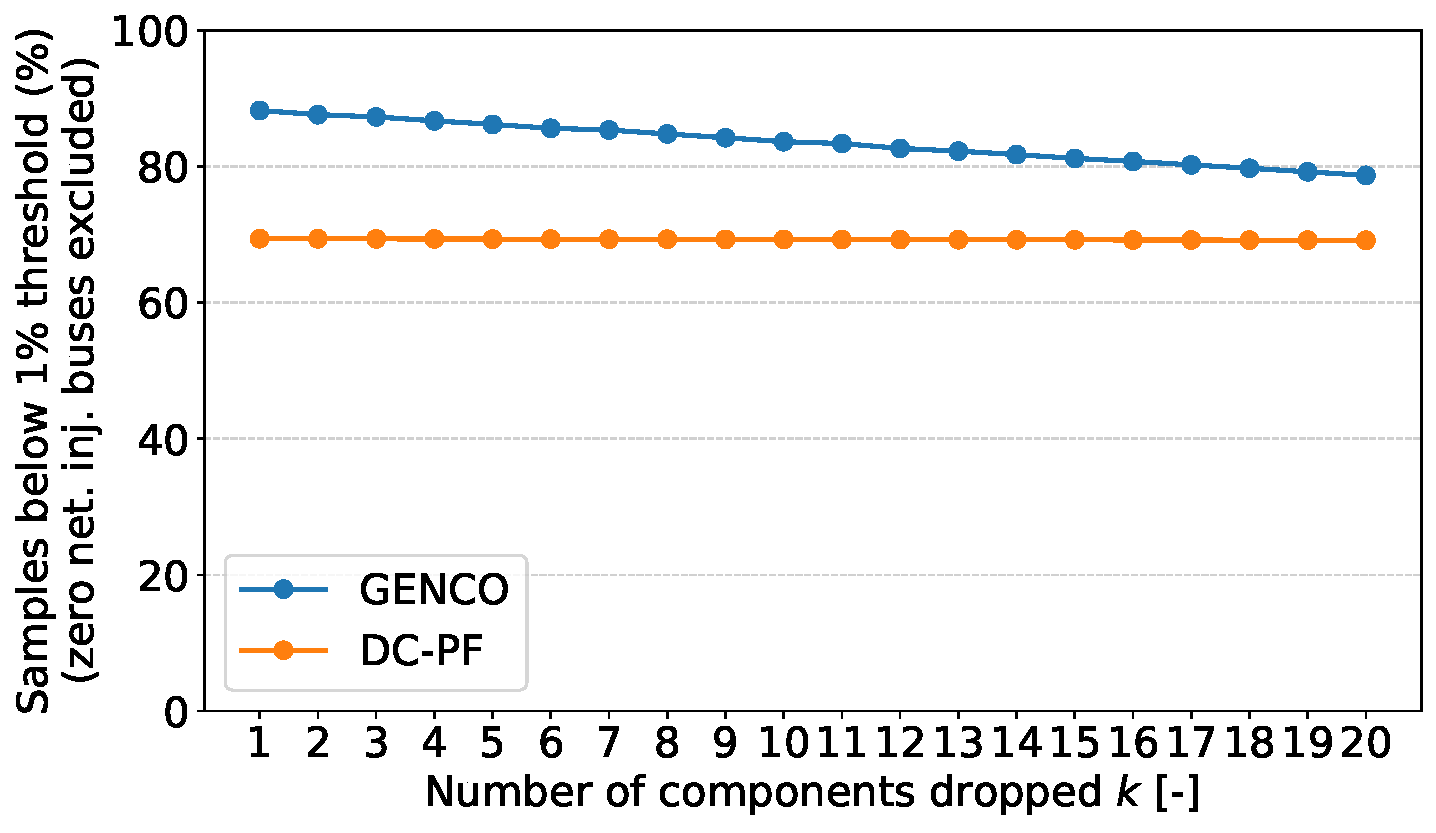
\includegraphics[width=\linewidth]{figures/robustness/below_1pct_threshold_vs_k.pdf}
\caption{Percentage of samples with relative active power-balance residual below 1\% as a function of contingency order $k$ (excluding zero-injection buses). The fraction decreases with $k$ for both methods, but remains consistently higher for \genco.}
\label{fig:rel_threshold_vs_k}
\end{minipage}

\end{figure}


\subsection{Residuals at Zero-Net-Injection Buses}
\label{appendix:zeroinj}

The distribution of bus-level absolute active power-balance residuals at zero-net-injection buses for \genco and DC-PF across $N$-$k$ contingencies with $k=1,\dots,20$ is shown in \cref{fig:zeroinj_boxplot}. Unlike the relative metric in the main text, this view isolates buses for which no normalization by net injection is possible and directly reports the remaining power-balance mismatch in MW.

\cref{fig:zeroinj_abs_threshold_k10} complements this distributional view with the percentage of zero-net-injection buses below practically relevant absolute residual thresholds at $k=10$. 

\begin{figure}[H]
\centering

\begin{minipage}{0.4\linewidth}
\centering
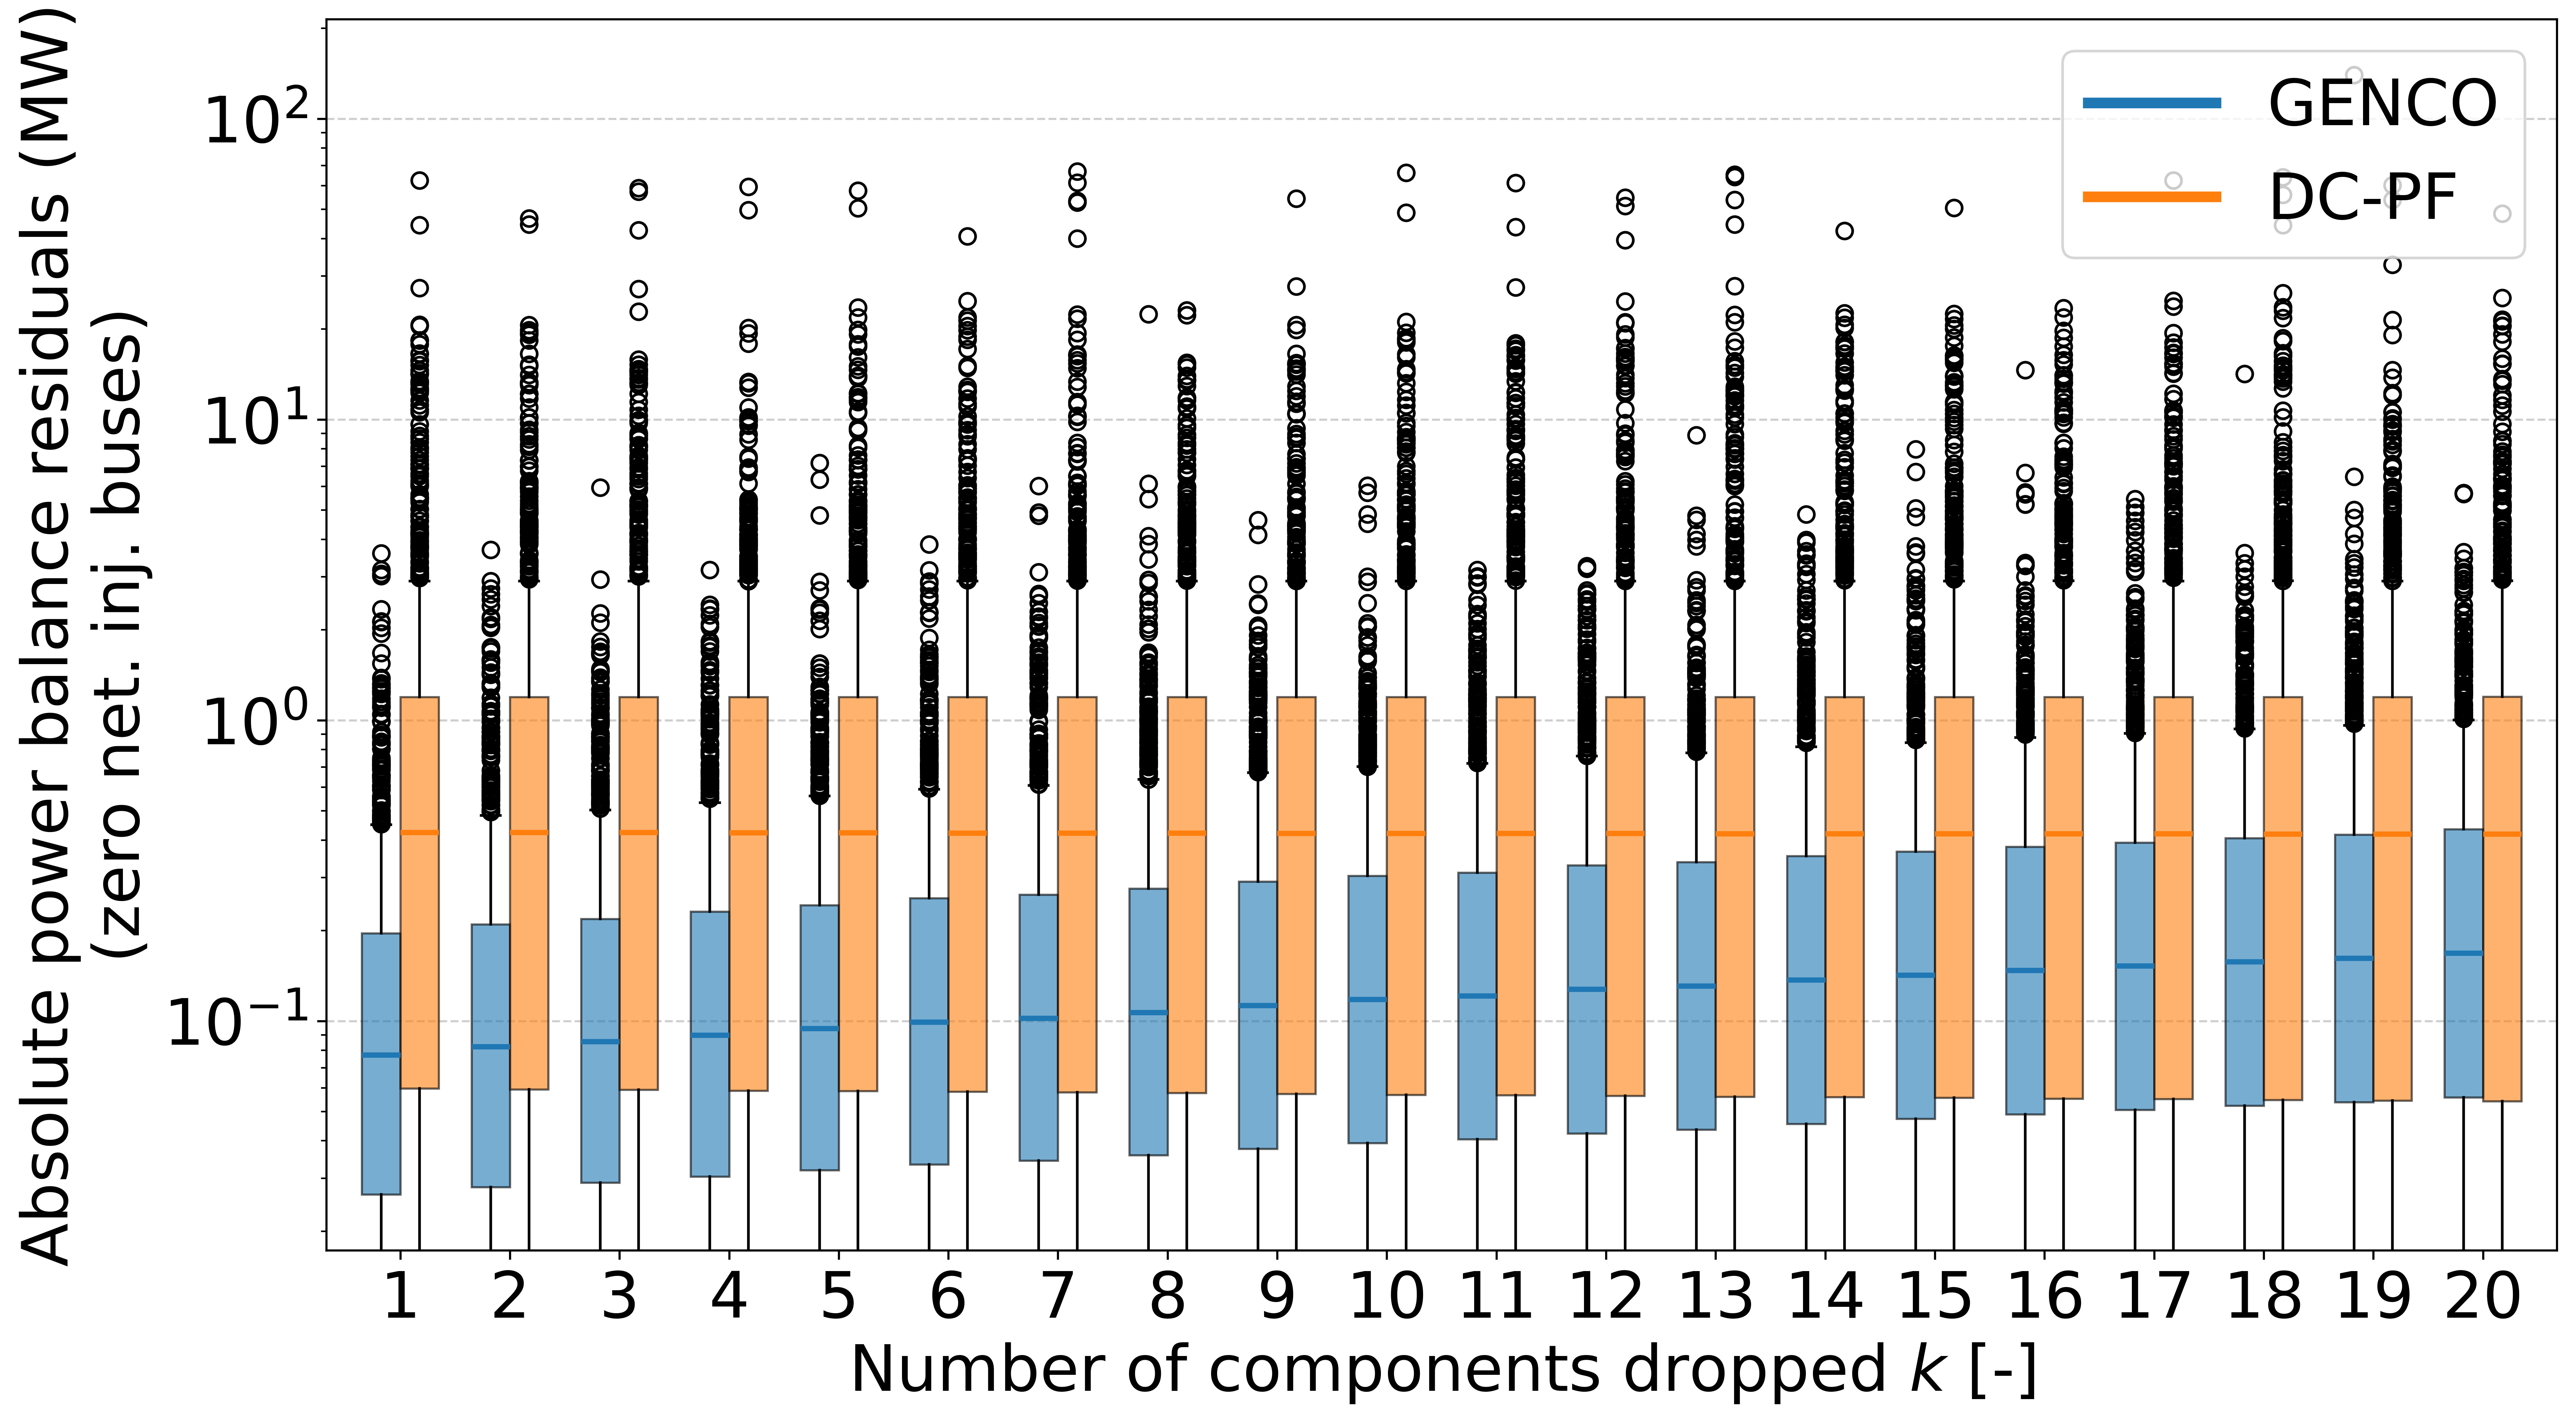
\includegraphics[width=\linewidth]{figures/robustness/boxplot_zero_inj_absolute_residuals.png}
\caption{Bus-level absolute active power-balance residuals at zero-net-injection buses under $N$-$k$ contingencies ($k=1,\dots,20$). \genco achieves consistently lower residuals than DC-PF across the entire distribution. Whiskers indicate 1.5$\times$IQR.}
\label{fig:zeroinj_boxplot}
\end{minipage}
\hspace{3cm}
\begin{minipage}{0.4\linewidth}
\centering
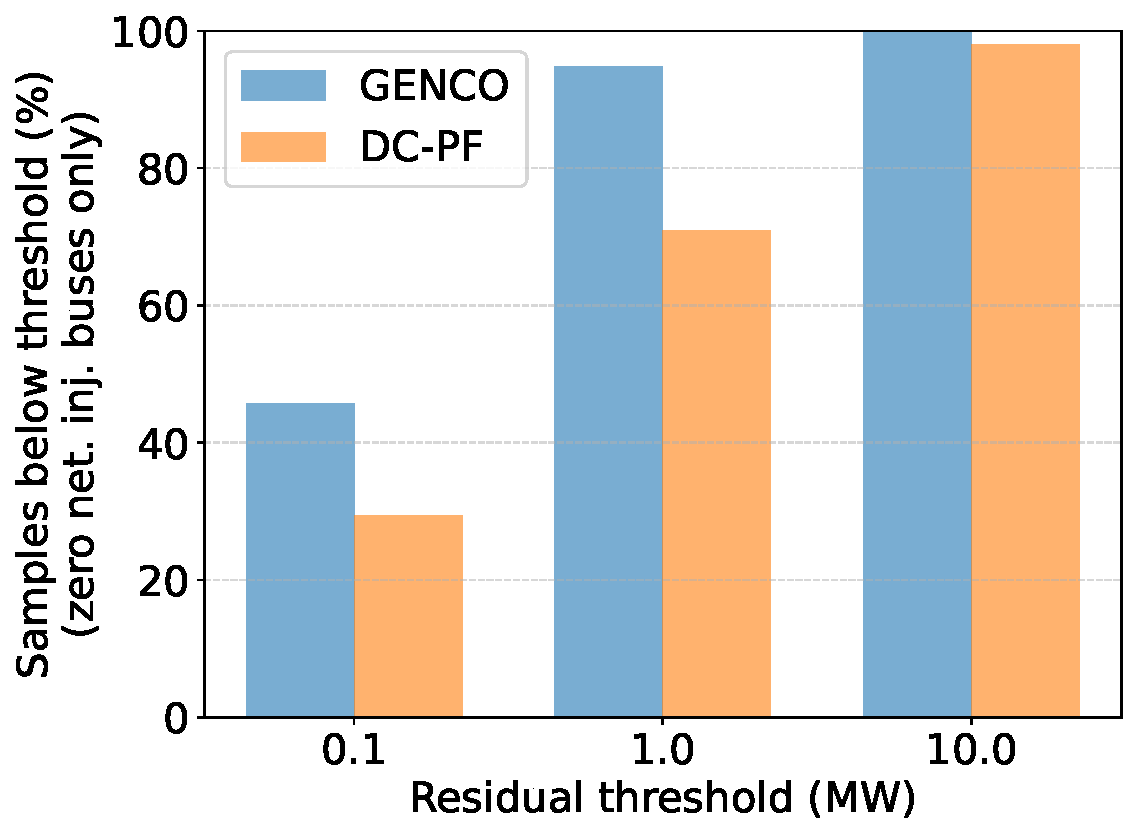
\includegraphics[width=\linewidth]{figures/robustness/threshold_share_absolute_k10_zero_inj.pdf}
\caption{Percentage of zero-net-injection buses below absolute active power-balance residual thresholds at $k=10$. \genco consistently achieves a higher fraction of low-residual predictions than DC-PF across all thresholds.}
\label{fig:zeroinj_abs_threshold_k10}
\end{minipage}

\end{figure}

\section{Voltage Prediction under Out-of-Limit Operating Conditions}
\label{appendix:voltage_violations}

Voltage violations are rare in the N-2 dataset, with only $6.9 \times 10^{-4}$\% of buses operating outside the nominal voltage range, i.e., 121 buses out of the 17,424,000 buses in the dataset. \cref{fig:genco_voltage} compares \genco voltage magnitude predictions against AC-PF across the full operating range, including undervoltage ($<0.9$~p.u.) and overvoltage ($>1.1$~p.u.) conditions. \genco remains closely aligned with the reference solution even in these rarely observed regimes.\\

Absolute voltage magnitude errors as a function of the true voltage magnitude are depicted in \cref{fig:voltage_boxplot}. Across all voltage ranges, including out-of-limit conditions, \genco maintains errors below 0.015~p.u. These results suggest that the model generalizes well to voltage violations despite their extreme scarcity in the training data, and does not require dedicated oversampling of such scenarios.


\begin{figure}[H]
\centering

\begin{minipage}{0.4\linewidth}
\centering
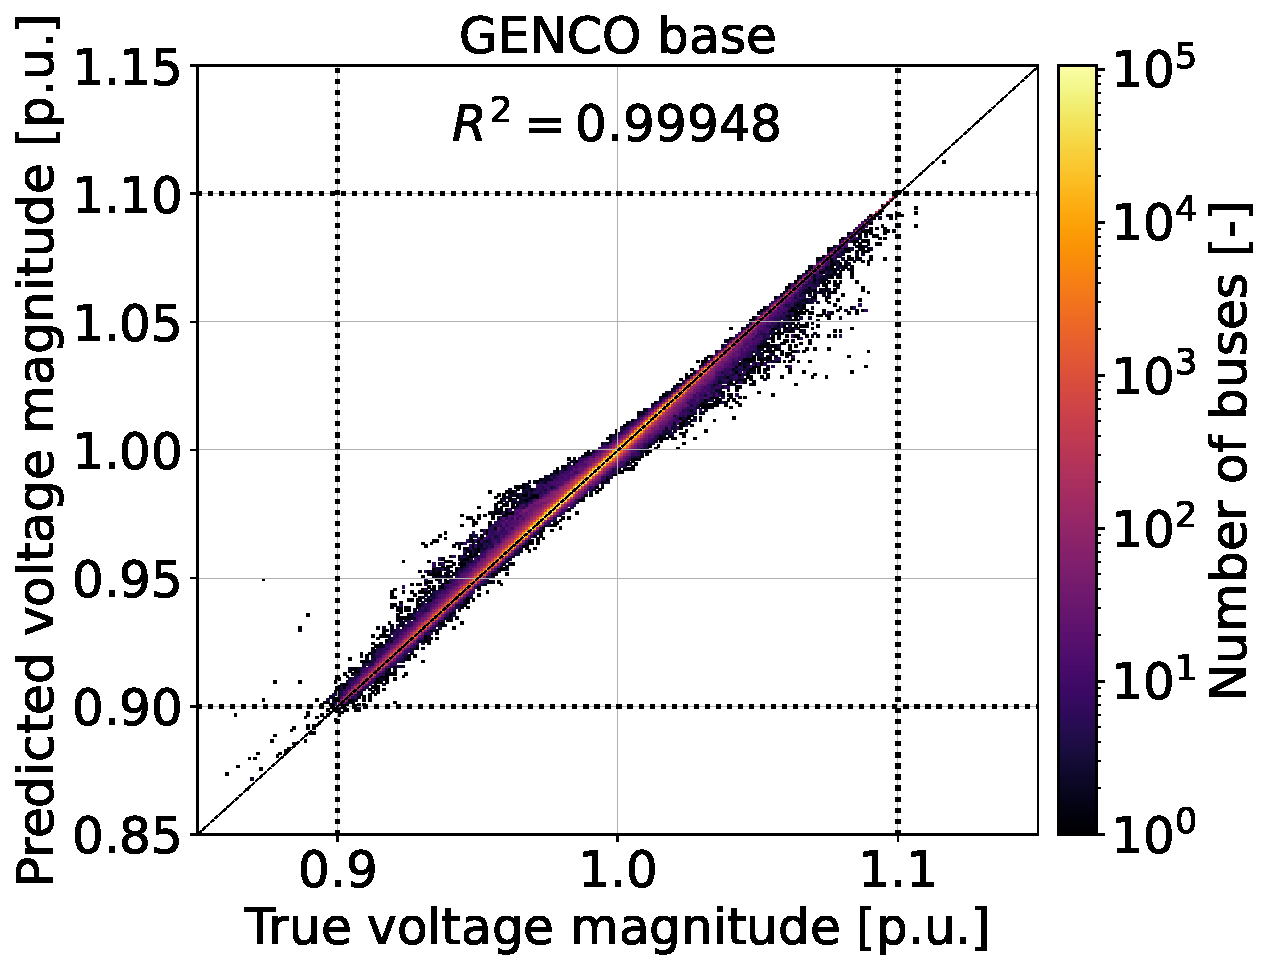
\includegraphics[width=\linewidth]{figures/robustness/mass_correlation_density_voltage_Texas.pdf}
\caption{Bus voltage predictions obtained with \genco compared to AC-PF voltages.}
\label{fig:genco_voltage}
\end{minipage}
\hspace{3cm}
\begin{minipage}{0.4\linewidth}
\centering
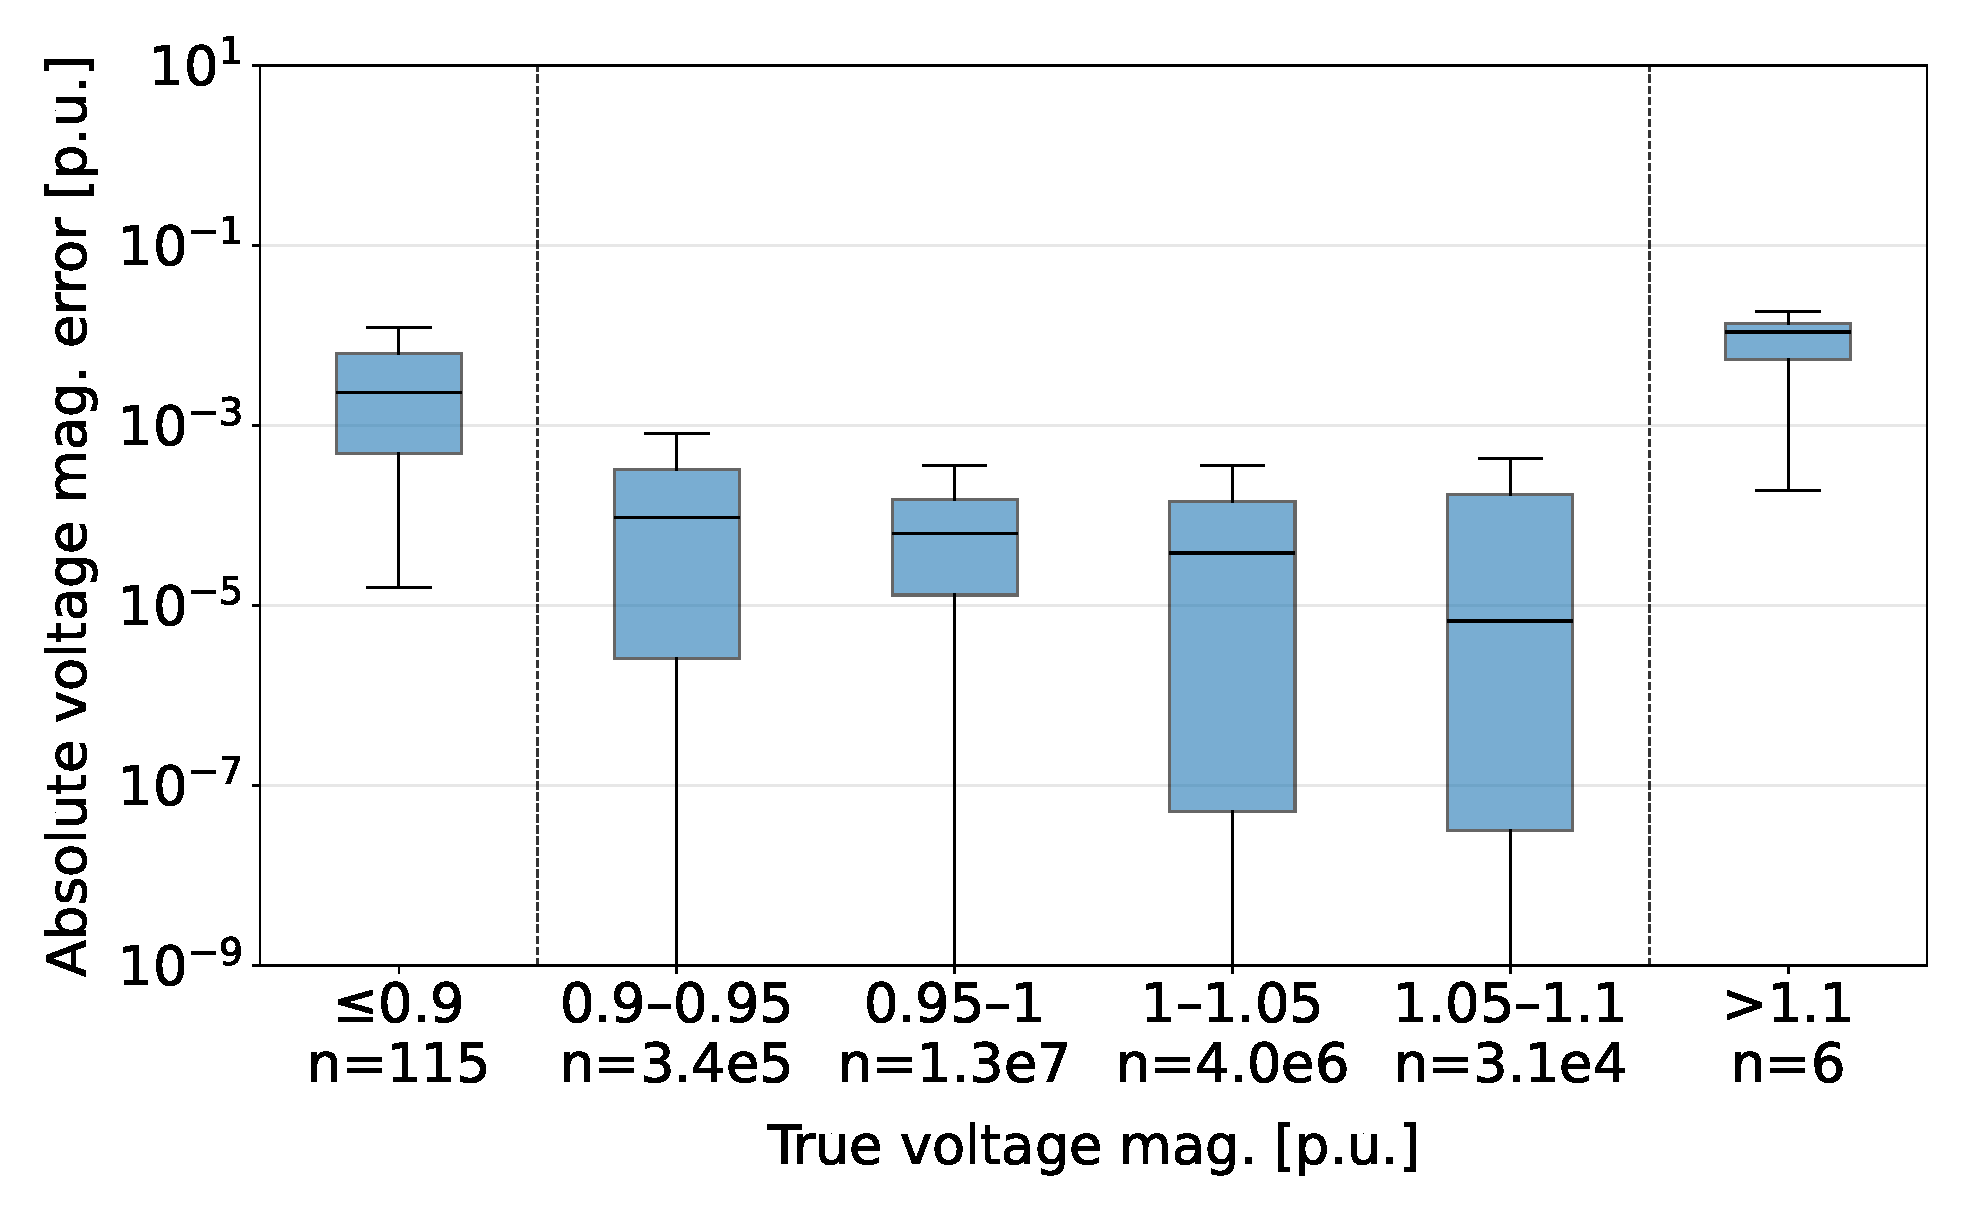
\includegraphics[width=\linewidth]{figures/robustness/voltage_error_boxplot_by_true_voltage_Texas.pdf}
\caption{Absolute voltage magnitude prediction error as a function of the true voltage magnitude. $n$ indicates the number of test samples in each bin.}
\label{fig:voltage_boxplot}
\end{minipage}

\end{figure}



\section{\textit{Supplementary Material for \cref{subsec:hq1200}: Results -- Validation on Real Data from the Hydro-Québec Grid}}
\label{appendix:hqgrit}

\paragraph{Additional details about GRIT-HQ.} GRIT-HQ builds on the GRIT architecture~\cite{ma2023graph}, which combines random-walk-based positional encodings, attention layers that jointly update node and edge representations, and explicit incorporation of node degree information at each layer. We adapt the original model based on a large-scale empirical study over 600,000 scenarios with graph sizes ranging from 24 to 240 nodes, which guided the choice of depth, width, and attention configuration. In this setting, we observe that relative random walk positional encodings (RRWP) provide negligible gains over random walk structural encodings (RWSE). We therefore adopt RWSE in the final model, which reduces memory complexity while preserving linear scaling with graph size. The resulting architecture operates on a homogeneous bus-level graph representation, consistent with the original GRIT formulation.


\section{\textit{Supplementary Material for \cref{sec:discussion}: Discussion}}
\label{appendix:future_work}

\subsection{Future Work to Advance GENCO's Performance}
To further strengthen \genco's utility, scalable long-range message-passing and attention mechanisms must be explored, and all OPF constraints must be incorporated into the loss at each correction step. For expansion-planning use cases, robustness to additional grid components and to load and generation increases must also be analyzed. All of these perturbations will be included in the next version of \datakit.

\subsection{Future Work to Advance GENCO's Deployment}
In \cref{subsec:comparison_data_hq}, we successfully validated the realism of synthetic data generated with \datakit against SCADA data from HQ1200 based on the normalized mean feature entropy of the entire grid. In the future, the analysis will be extended to a finer level of granularity, as initial observations from HQ1200 indicate clustered topology changes rather than the uniformly distributed perturbations currently generated by \datakit. Further, analyzing model uncertainty conditioned on specific perturbations opens the door to uncertainty bounds based on conformal prediction, as demonstrated in~\cite{alcantara2026trustworthinesslayerfoundationmodels}.\\

In \cref{subsec:generalization}, we demonstrated \genco's robustness to contingencies of up to $N$-$20$ and out-of-operating-limit scenarios. However, for the most demanding case of entirely unseen grids, even our subgrid-based pre-training strategy (\cref{subsubsec:transfer}) achieved moderate performance, with zero-shot residuals exceeding those of DC solvers. Accordingly, improved training strategies that yield acceptable zero-shot performance will be explored to eliminate the need for model fine-tuning.

\subsection{Future Work to Advance Standardized Development and Benchmarking}
So far, we have benchmarked \genco's runtime against classical solvers and its accuracy against other neural solvers on \pfdelta and OPFData with limited perturbation diversity. In the future, third-party neural solvers must therefore be onboarded to \graphkit and evaluated on our diverse synthetic \datakit benchmark using the hardware configuration reported in this work. \\

Moreover, residuals and violations must be reported using relative metrics rather than absolute quantities such as MW and MVar. For example, power balance errors must be normalized by the corresponding net injections, and branch flow violations by their thermal limits, as absolute errors can have very different implications depending on the scale of the underlying grid element. Finally, reporting violation rates across multiple thresholds and full error distributions, rather than only averages, will enable more meaningful robustness comparisons.

\section{Code \& Reproducibility}

\graphkit, \genco (implemented in \graphkit), and \datakit continue to evolve beyond this paper, and their latest versions are available on \href{https://github.com/gridfm}{GitHub}. The scripts, configuration files, library versions, and trained models used for the results in this paper are released separately from those development branches. Step-by-step guides for each experiment are at \href{https://github.com/albanpuech/GENCO/tree/main/repro_instructions}{\texttt{repro\_instructions}}. The code and configs are on the \texttt{genco-paper-repro} branch of \href{https://github.com/gridfm/gridfm-graphkit/tree/genco-paper-repro}{\graphkit} and \href{https://github.com/gridfm/gridfm-datakit/tree/genco-paper-repro}{\datakit}. \Cref{subsec:pf} uses \href{https://github.com/gridfm/gridfm-graphkit/tree/genco-paper-repro-pfdelta}{\texttt{genco-paper-repro-pfdelta}}, and the subgrid pretraining run in \cref{subsubsec:transfer} uses \href{https://github.com/gridfm/gridfm-graphkit/tree/genco-paper-repro-pretraining}{\texttt{genco-paper-repro-pretraining}}. Checkpoints are on \href{https://huggingface.co/gridfm}{Hugging Face} under \texttt{gridfm/genco-pfdelta}, \texttt{gridfm/genco-opfdata}, \texttt{gridfm/genco-pf-datakit}, \texttt{gridfm/genco-opf-datakit}, \texttt{gridfm/genco-pf-contingency}, and \texttt{gridfm/genco-pf-transfer}. The datasets used for training, evaluation, pretraining, and the runtime measurements are in the same organization.
